% presentation
\documentclass{beamer}

\usetheme{Warsaw}

% rus lang
\usepackage[main=russian,english]{babel}

% insert images
\usepackage{wrapfig}
\usepackage{graphicx}

% declare operator
\DeclareMathOperator*{\argmin}{argmin} % thin space, limits underneath in displays
\newcommand{\at}[2][]{#1|_{#2}}

% alrorithm
\usepackage{algorithm2e}
\usepackage{algorithm}
\usepackage{algpseudocode}
% \usepackage{algorithmic}

% math
\newtheorem{rustheorem}{Теорема}
\usepackage{amsmath}
\DeclareMathOperator{\sign}{sign}
\DeclareMathOperator{\K}{K}

\title[Метрики]{Лекция 5. Оценка качества моделей}
\subtitle{Основы интеллектуального анализа данных}
\author{Полузёров Т. Д.}
\institute{БГУ ФПМИ}
\date{}

\begin{document}
	
	\begin{frame}
		\titlepage
	\end{frame}
	
	\section{Обобщаяющая способость}
	
	\subsection{Функция потерь}
	
	\begin{center}
		\frametitle{Структура лекции}
		\tableofcontents	
	\end{center}

	\begin{frame}
		\frametitle{Дано}
		Имеется выборка объектов $X = (x_1, ..., x_{\ell}), X \in \mathbb{X}$ и соответствующие им метки $Y = (y_1, ..., y_{\ell}), Y \in \mathbb{Y}$.
		
		\vspace{5pt}
		
		Построена модель $a: \mathbb{X} \rightarrow \mathbb{Y}$ по данным $D^{\ell} = (X, Y)$ с~помощью метода обучения $\mu: \mathbb{X} \times \mathbb{Y} \rightarrow \mathbb{A}$ -- минимизации эмперического риска
		\[
		Q(a, D^{\ell}) = \frac{1}{\ell} \sum_{i=1}^{\ell} \mathcal{L}(y_i, a(x_i, \theta))
		\rightarrow \min_{\theta}
		\]
		где $\mathcal{L}: \mathbb{Y} \times \mathbb{Y} \rightarrow \mathbb{R}$ - функция ошибки модели на объекте
		
		\vspace{15pt}
		
		Насколько адекватно работает модель \textbf{на других объектах} из~$\mathbb{X}$?	
	\end{frame}
	
	\begin{frame}
		\frametitle{Обобщаяющая способность}
		
		Обобщающая способность алгоритма $a$
		\[
		G(a) = E_{\mathbb{X}}\{\mathcal{L}(y, a(x))\}
		\]
		
		На практике используется эмпирическая оценка   
		\[
		\hat{G}(a) = 
		Q(a, \acute{D}) 
		= \frac{1}{|\acute{D}|} 
		\sum_{i=1}^{|\acute{D}|} 
		\mathcal{L}(y_i, a(x_i))
		\]
		
		показывает среднюю ошибку модели $a$, обученной по выборке $D$, на других данных $\acute{D} \in (\mathbb{X} \times \mathbb{Y})$.
		
		При $|\acute{D}| \rightarrow \infty$, согласно закону больших чисел, $\hat{G} \rightarrow G$ .
	\end{frame}
	
	\begin{frame}
		\frametitle{Метод отложенной выборки}
		Случайное разбиение выборки $D = D_{train} \sqcup D_{test}$.
		
		Обучение на $D_{train}$, а оценка на $D_ {test}$.
		
		\[
		\hat{G}(a) = Q(\mu(D_{train}), D_{test})
		\]
		
		\begin{itemize}
		\item Обычно пропорции train - 80\%, test- 20\%		
		\item Для задачи классификации случайное разбиение сохраняющее пропорции классов -- \textbf{стратифицированное}
		\item Вычислительно эффективно -- всего 1 обучение
		\item Может быть нестабильной оценкой
		\end{itemize}
	\end{frame}
	
	\subsection{Понятие метрики}
		
	\begin{frame}
		\frametitle{Функция потерь $\ne$ метрика качества}
		Имея алгоритм $a$ хочется оценить его реальный бизнес эффект. Метрика $\mathcal{M}$ отражает целевой эффект от модели $a$. Может порождаться иерархия метрик.
		
		\vspace{15pt}
		
		Пример иерархии метрик для задачи рекомендаций фильмов:
		\begin{enumerate}
			\item Доход сервиса -- глобальная цель
			\item Среднее число просматриваемых фильмов в неделю -- косвенный показатель релевантности рекомендаций
			\item Точность классификации <кликнет - не кликнет> -- можно рассчитать по имеющимся данным
			\item Функция потерь ($\mathcal{L}$) -- по ней и строим модель $a$
		\end{enumerate}
	\end{frame}
	
	\begin{frame}
		\frametitle{Функция потерь как апроксимация метрики}
		Метрика $\mathcal{M}$ - внешний, объективный показатель качества алгоритма. 
		
		Функция потерь $\mathcal{L}$ - математически удобная функция, которая служит лишь для построения алгоритма.
		
		\vspace{15pt}
		\begin{itemize}
			\item Глобальная задача стоит в оптимизации метрики, а функция потерь выступает как прокси.
			\item В некоторых задачах они могут совпадать - тогда метрика оптимизируется напрямую.
			\item Прямые верхнеуровневые метрики бывает невозможно измерить в моменте, поэтому используются косвенные
		\end{itemize}
	\end{frame}
	
	\begin{frame}
		\frametitle{Online и Offline метрики}
		\textbf{Online} - метрики, которые рассчитываются по уже работающей системе.
		
		\textbf{Offline} - рассчитываются до введения в эксплуатацию, могут быть рассчитаны по имеющимся данным.
 		
 		\vspace{15pt}
 		
 		На этапе построении моделей и их сравнения доступны только оффлайн метрики. $(X, Y) \in (\mathbb{X}, \mathbb{Y})$, $\mathcal{M}: \mathbb{Y} \times \mathbb{Y} \rightarrow \mathbb{R}$
	\end{frame}
	
	\section{Метрики классификации}
		
	\subsection{Метки классов}
	
	\begin{frame}
		\frametitle{Доля ошибочных классификаций}
		
		\textbf{Доля ошибочных классификаций} (Accuracy):
		\[
		Accuracy(y, \hat{y}) = \frac{1}{\ell} \sum_{i}^{N} [y_i = \hat{y}_i]
		\]
		
		Или сопряженная с ней \textbf{доля ошибочных классификаций} (Error Rate):
		\[
		ErrorRate = 1 - Accuracy
		\]
		
		\begin{itemize}
			\item неприменима при сильном диссбалансе классов
			\item не учитываеь величину ошибки на объектах разных классов
		\end{itemize}
	\end{frame}
	
	\begin{frame}
		\frametitle{Матрица ошибок}
		\textbf{Матрица ошибок} (Confusion Matrix) -- кросс-таблица из истинных меток и прогнозов.
		
		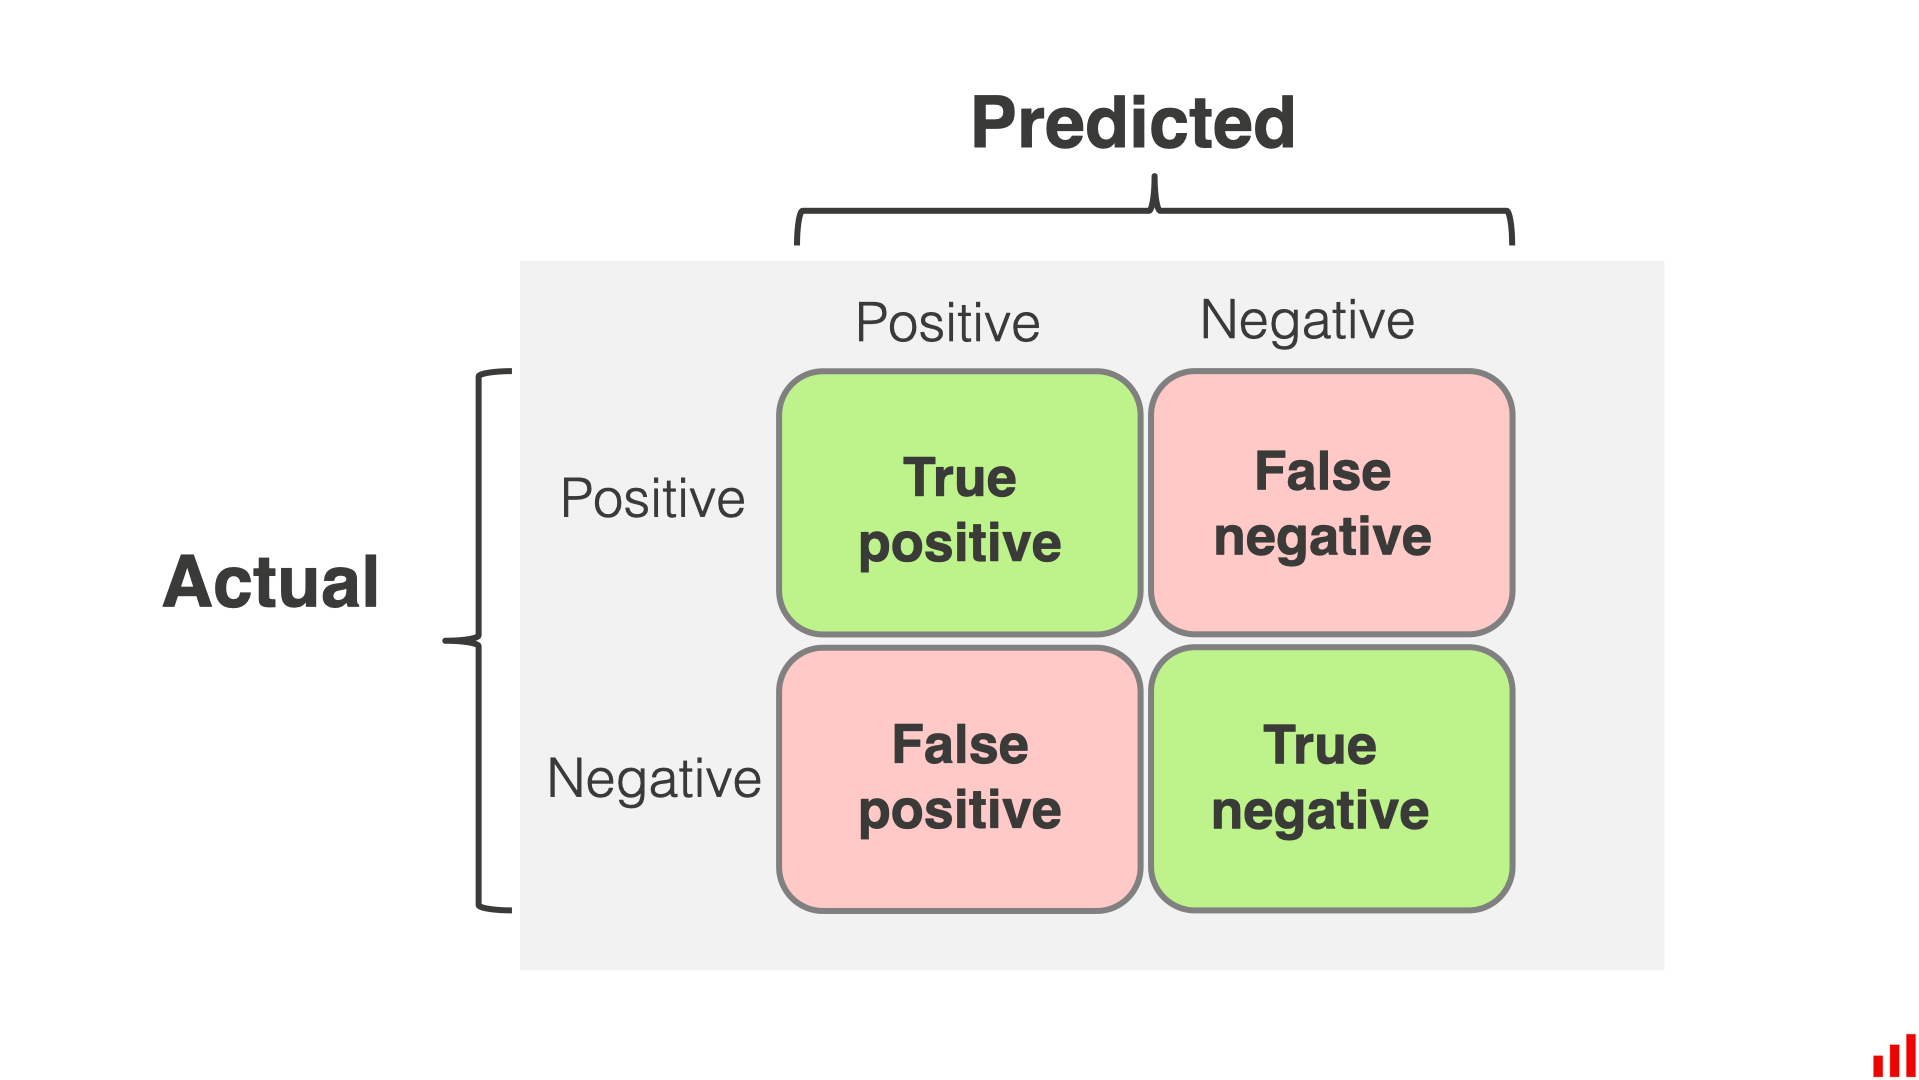
\includegraphics[width=1.1\textwidth]{img/confusion_matrix.png}
	\end{frame}

	\begin{frame}
		\frametitle{Элементы матрицы ошибок}
		True/False - допустил ли классификатор ошибку
		
		Positive/Negative - ответ классификатора
		
		\vspace{15pt}
		
		\begin{itemize}
			\item TP - верно определенный положительный класс
			\item TN - верный негативный класс
			\item FP - ложное срабатывание (ошибочная положительная классификация)
			\item FN - пропуск объекта(ошибочное не срабатывание)
		\end{itemize}
		
		\vspace{10pt}
		
		\[
		Accuracy = \frac{TP + FP}{TP + TN + FP + FN}
		\]
	\end{frame}
	
	\begin{frame}
		\frametitle{Метрики по матрице ошибок}
		\textbf{Ошибка 1-го рода}(False Positive Rate, FPR). Вероятность~ложного срабатывания: 
		\[
		P(\hat{y}=+1 | y = -1) = \frac{FP}{FP + TN}
		\]
		\textbf{Ошибка 2-го рода}(False Negative Rate, FNR). Вероятность~пропуска:
		\[
		P(\hat{y}=-1 | y = +1) = \frac{FN}{FN + TP}
		\]
	\end{frame}
	
	\begin{frame}
		\frametitle{Точность и полнота}
		
		\textbf{Точность} -- доля верных классификаций при срабатывании
		\[
		Precision = \frac{TP}{TP + \textbf{FP}}
		\]
		
		\textbf{Полнота} -- доля всех положительных объектов на которых сработал классификатор
		\[
		Recall = \frac{TP}{TP + \textbf{FN}}
		\]
	\end{frame}
	
	\begin{frame}
		\frametitle{Усреднение точности и полноты}
		Одновременно учитывать Precision и Recall можно с помощью среднего гармонического:
		\[
		F_1 = \frac{2}{\frac{1}{Precision} + \frac{1}{Recall}} =
		2 \frac{Precision \cdot Recall}{Precision + Recall}
		\]
		
		Важность одной из метрик можно учесть с помощью коэффициента $\beta$
		\[
		F_{\beta} = (\beta^2 + 1) \frac{Precision \times Recall}{Precision + \beta^2 Recall}
		\]
	\end{frame}
	
	\begin{frame}
		\frametitle{Линии уровня}
		
		\begin{columns}
			\begin{column}{0.5\textwidth}
				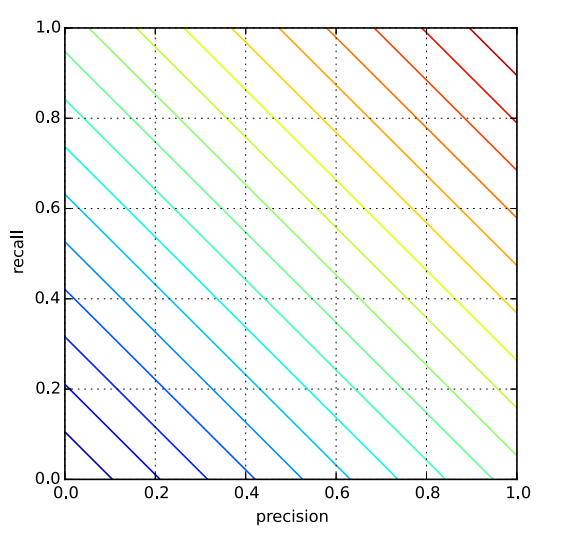
\includegraphics[width=\textwidth]{img/fbeta_avg.png}
				
				Среднее арифметическое
			\end{column}
			\begin{column}{0.5\textwidth}
				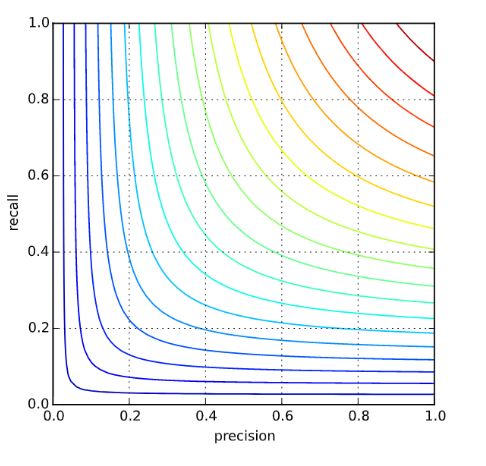
\includegraphics[width=\textwidth]{img/fbeta_harm.png}
				Среднее гармоническое
			\end{column}
		\end{columns}
		
	\end{frame}
	
	\subsection{Порядок объектов}
	
	\begin{frame}
		\frametitle{Порог классификации}
		Классификаторы вида $a(x, t) = \sign \left(f(x) - t\right)$ допускают настройку порога отсечения $t$.
		
		\vspace{15pt}
		
		При $t \rightarrow -\infty$:
		\begin{enumerate}
			\item все объекты классифицируются в \textbf{положительный} класс
			\item $Recall = 1$
			\item $Precision = $ доле положительных объектов в выборке
		\end{enumerate}
		
		\vspace{5pt}
		
		При $t \rightarrow +\infty$:
		\begin{itemize}
			\item  все объекты классифицируются в \textbf{отрицательный} класс
			\item $Recall = 0$
			\item $Precision$ - не определен
		\end{itemize}
	\end{frame}
	
	\begin{frame}
		\frametitle{Precision-Recall кривая}
		
		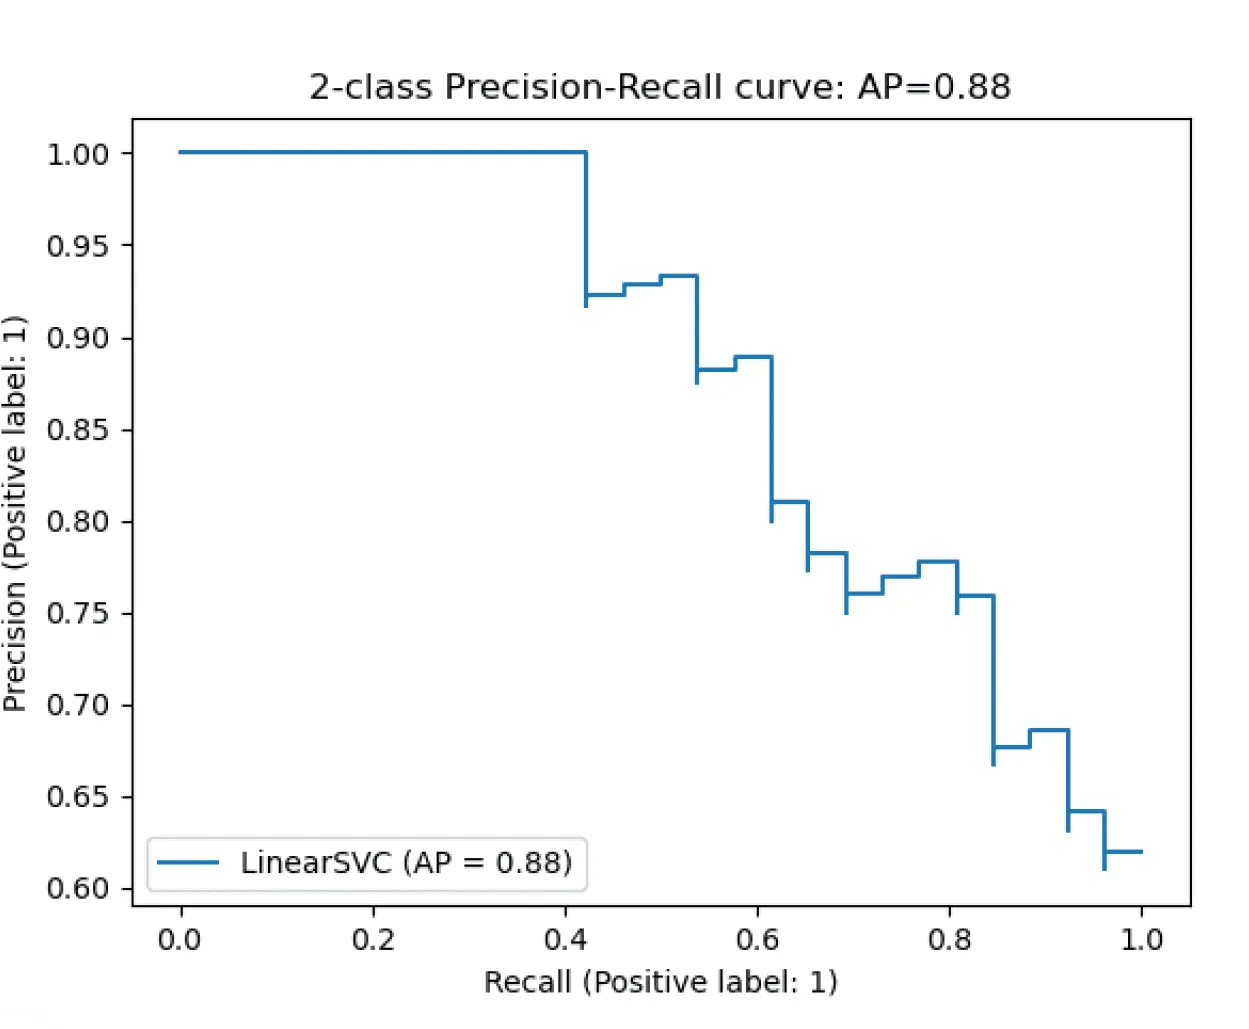
\includegraphics[width=0.9\textwidth]{img/pr_rc.png}
	\end{frame}
	
	\begin{frame}
		\frametitle{Зависимость от порога}
		
		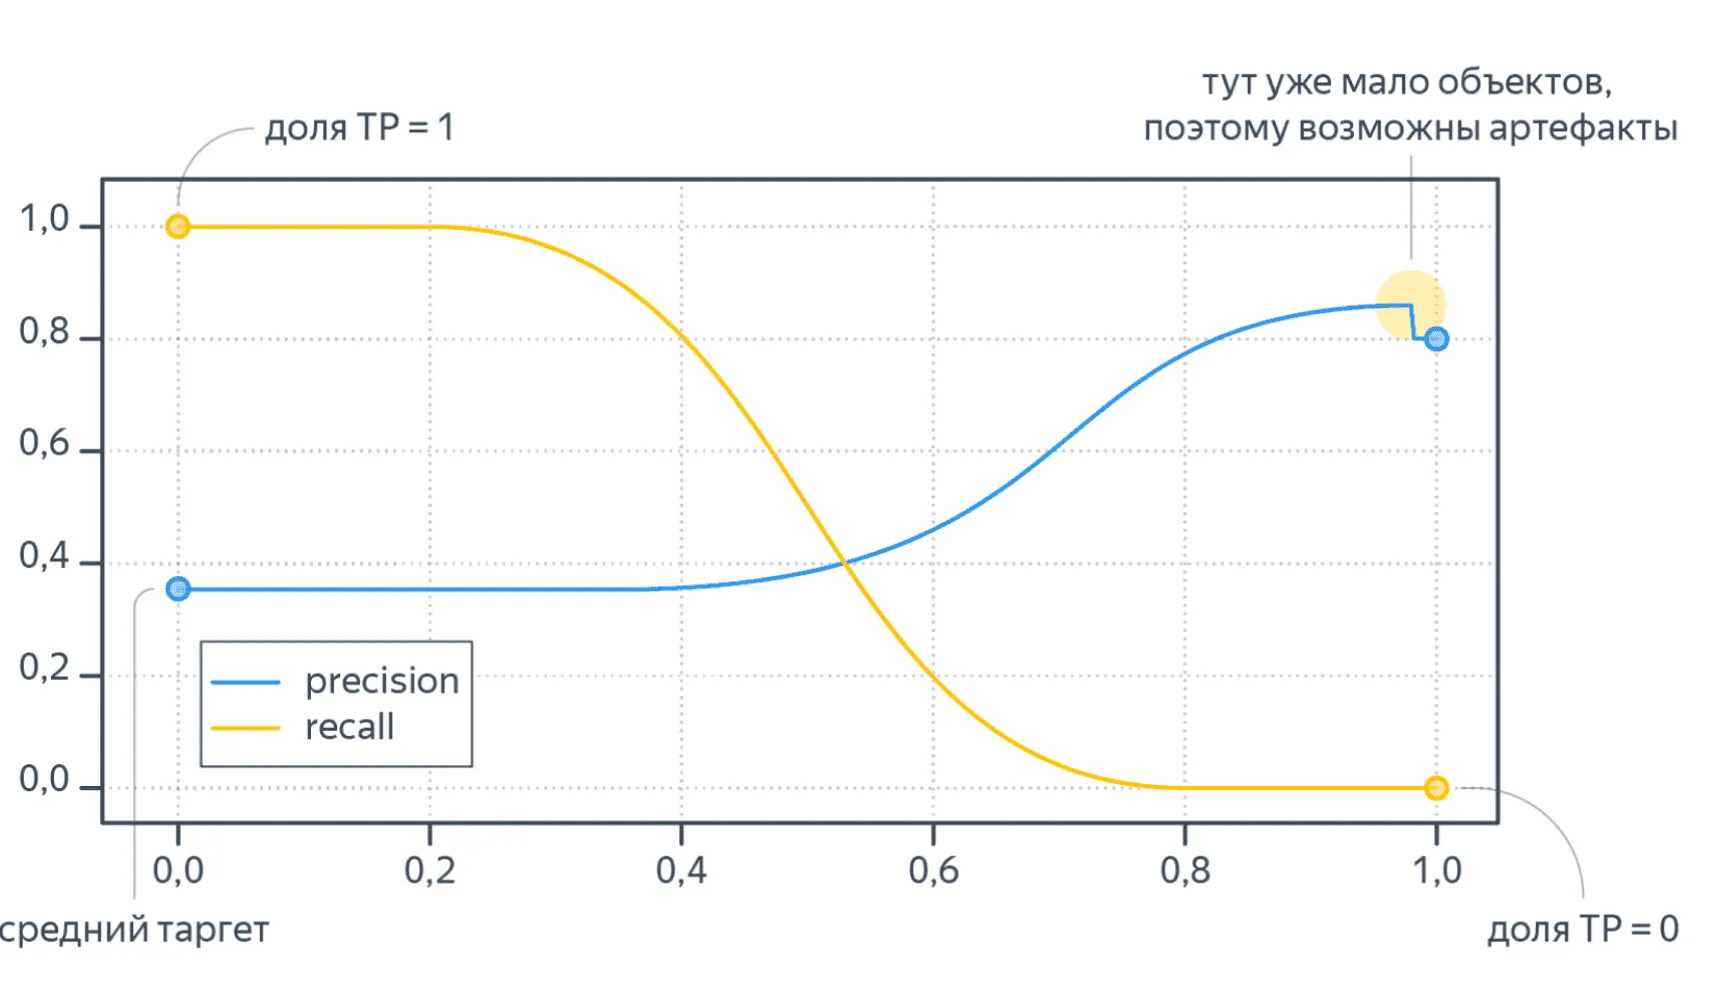
\includegraphics[width=1\textwidth]{img/pr_rc_th.png}
	\end{frame}
	
	\begin{frame}
		\frametitle{Оптимизация порога}
		Перебирая порог $t$ можно добиться \textbf{любого значения} $Recall \in [0, 1]$. При этом будет достигаться некоторый $Precision$. 
		
		\vspace{15pt}
		
		Оптимизация $Precision-Recall$ соотношения происходит так:
		\begin{enumerate}
			\item Строится алгоритм базовый алгоритм $b: \mathbb{X} \rightarrow \mathbb{R}$
			\item по отдельной валидационной выборке строятся кривые порога $t$
			\item определяется оптимальное соотношение Precision и Recall при $t^{*}$
			\item фиксируется итоговый алгоритм $a(x) = \sign \left( b(x) - t^{*} \right)$
		\end{enumerate} 
	\end{frame}
	
	\begin{frame}
		\frametitle{Средняя точность}
		Существует ряд метрик отражающих общее качество модели, инвариантно относительно порога $t$. 
		
		\[
		AveragePrecision = \int_{0}^{1} p(r) dr
		\]
		где $p(r)$ - значение $Precision$ при $Recall = r$.
		
		\vspace{15pt}
		
		Эта метрика соответствует площади под P-R кривой.
		
	\end{frame}
	
	\begin{frame}
		\frametitle{ROC-кривая}
		 TPR (True Positive Rate) - полнота (Recall)
		 
		 FPR (False Positive Rate) - доля отрицательных объектов на которых ложно сработал классификатор
		 
		 \begin{columns}
		 	\begin{column}{0.5\textwidth}
		 		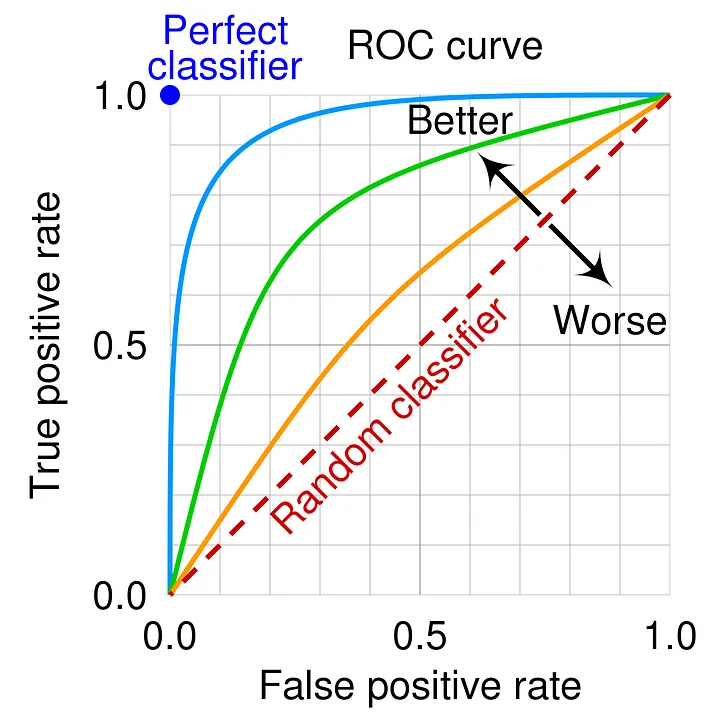
\includegraphics[width=0.9\textwidth]{img/roc.png}		
		 	\end{column}
		 	\begin{column}{0.5\textwidth}
		 		\[
		 		TPR = \frac{TP}{TP + NP}
		 		\]
		 		
		 		\[
		 		FPR = \frac{FP}{FP + TN}
		 		\]
		 	\end{column}
		 \end{columns}
	\end{frame}
	
	\begin{frame}
		\frametitle{Алгоритм построения ROC}
		
		\begin{enumerate}
			\item сортируем объекты по уверенности классификатора
			\item стартуем из точки (0, 0) и перебираем объекты выборки
			\item делаем шаг в 
			\begin{itemize}
				\item вверх, если объект правильно классифицирован
				\item право, если допущена ошибка
			\end{itemize}
		\end{enumerate}
	\end{frame}
	
	\section{Метрики регрессии}
	
	\subsection{Абсолютные}
	
	\begin{frame}
		\frametitle{Классика}
		Стандартный набор метрик в задачах регрессии
		
		\vspace{15pt}
		\begin{enumerate}
			\item 
			Средний квадрат ошибки
			\[
			MSE = \frac{1}{\ell}\sum_{i=1}^{\ell} (y_i - \hat{y}_i)^2
			\]
			\item
			Иногда MSE приводят к той же размерности что и ответы
			\[
			RMSE = \sqrt{MSE}
			\]
			\item 
			Средняя абсолютная ошибка
			\[
			MAE = \frac{1}{\ell}\sum_{i=1}^{\ell} |y_i - \hat{y}_i|
			\]
		\end{enumerate}
	\end{frame}
	
	\subsection{Относительные}
	
	\begin{frame}
		\frametitle{Относительные ошибки}
		
		Mean Absolute Percentage Error
		\[
		MAPE = \frac{1}{\ell} \sum_{i=1}^{\ell} \frac{|y_i - \hat{y}_i|}{|y_i|}
		\]
		
		Symmetric MAPE
		\[
		SMAPE = \frac{1}{\ell} \sum_{i=1}^{\ell} \frac{2 |y_i - \hat{y}_i|}{y_i + \hat{y}_i}
		\]
		
		Weighted Average PE
		\[
		WAPE = \sum_{i=1}^{\ell} \frac{|y_i - \hat{y}_i|}{\sum_{i=1}^{\ell} |y_i|}
		\]
	\end{frame}

	\section{Подбор гиперпараметров}
	
	\begin{frame}
		\frametitle{Подбор гиперпараметров}
		Параметры в модели бывают двух типов:
		\begin{enumerate}
			\item Параметры - те, что настраиваются в ходе решения $Q \rightarrow \min$
			\item Гиперпараметры - фиксируются до обучения 
		\end{enumerate}
		
		\vspace{15pt}
		
		\textit{Пример:}
		\[
		a_{d}(x, \omega) = \omega_0 + \omega_1 x + ... + \omega_d x^d
		\]
		$\omega$ - параметры, а $d$ - гиперпараметр
		
		\vspace{15pt}
		
		Как определить оптимальные значения гиперпараметров?
	\end{frame}
	
	\begin{frame}
		\frametitle{Отложенные выборки}
		
		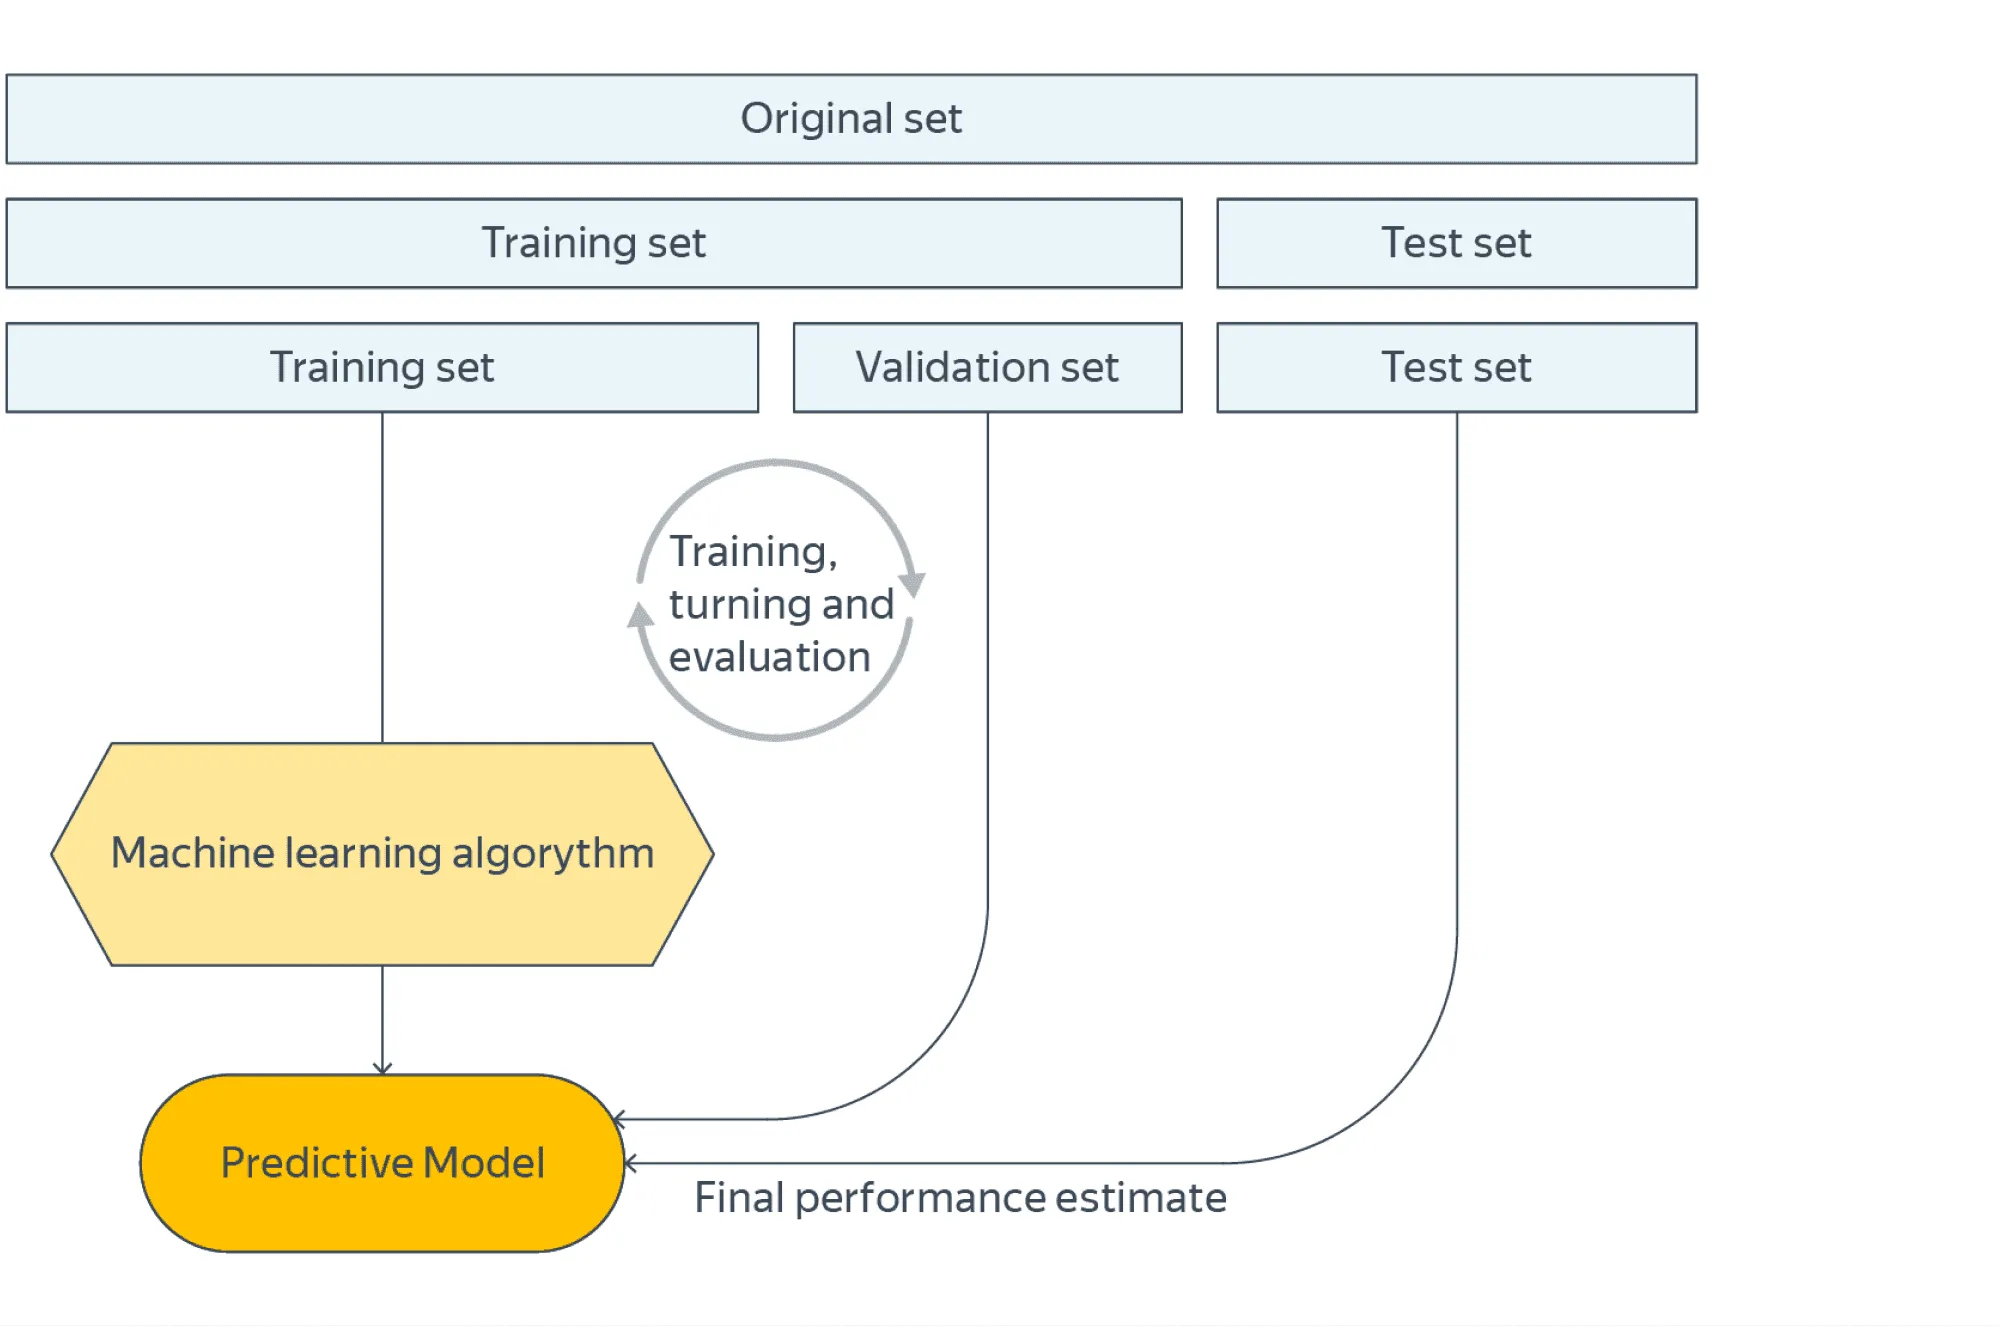
\includegraphics[width=1\textwidth]{img/tvt_split.png}
	\end{frame}
	
	\begin{frame}
		\frametitle{Кросс-валидация}
		
		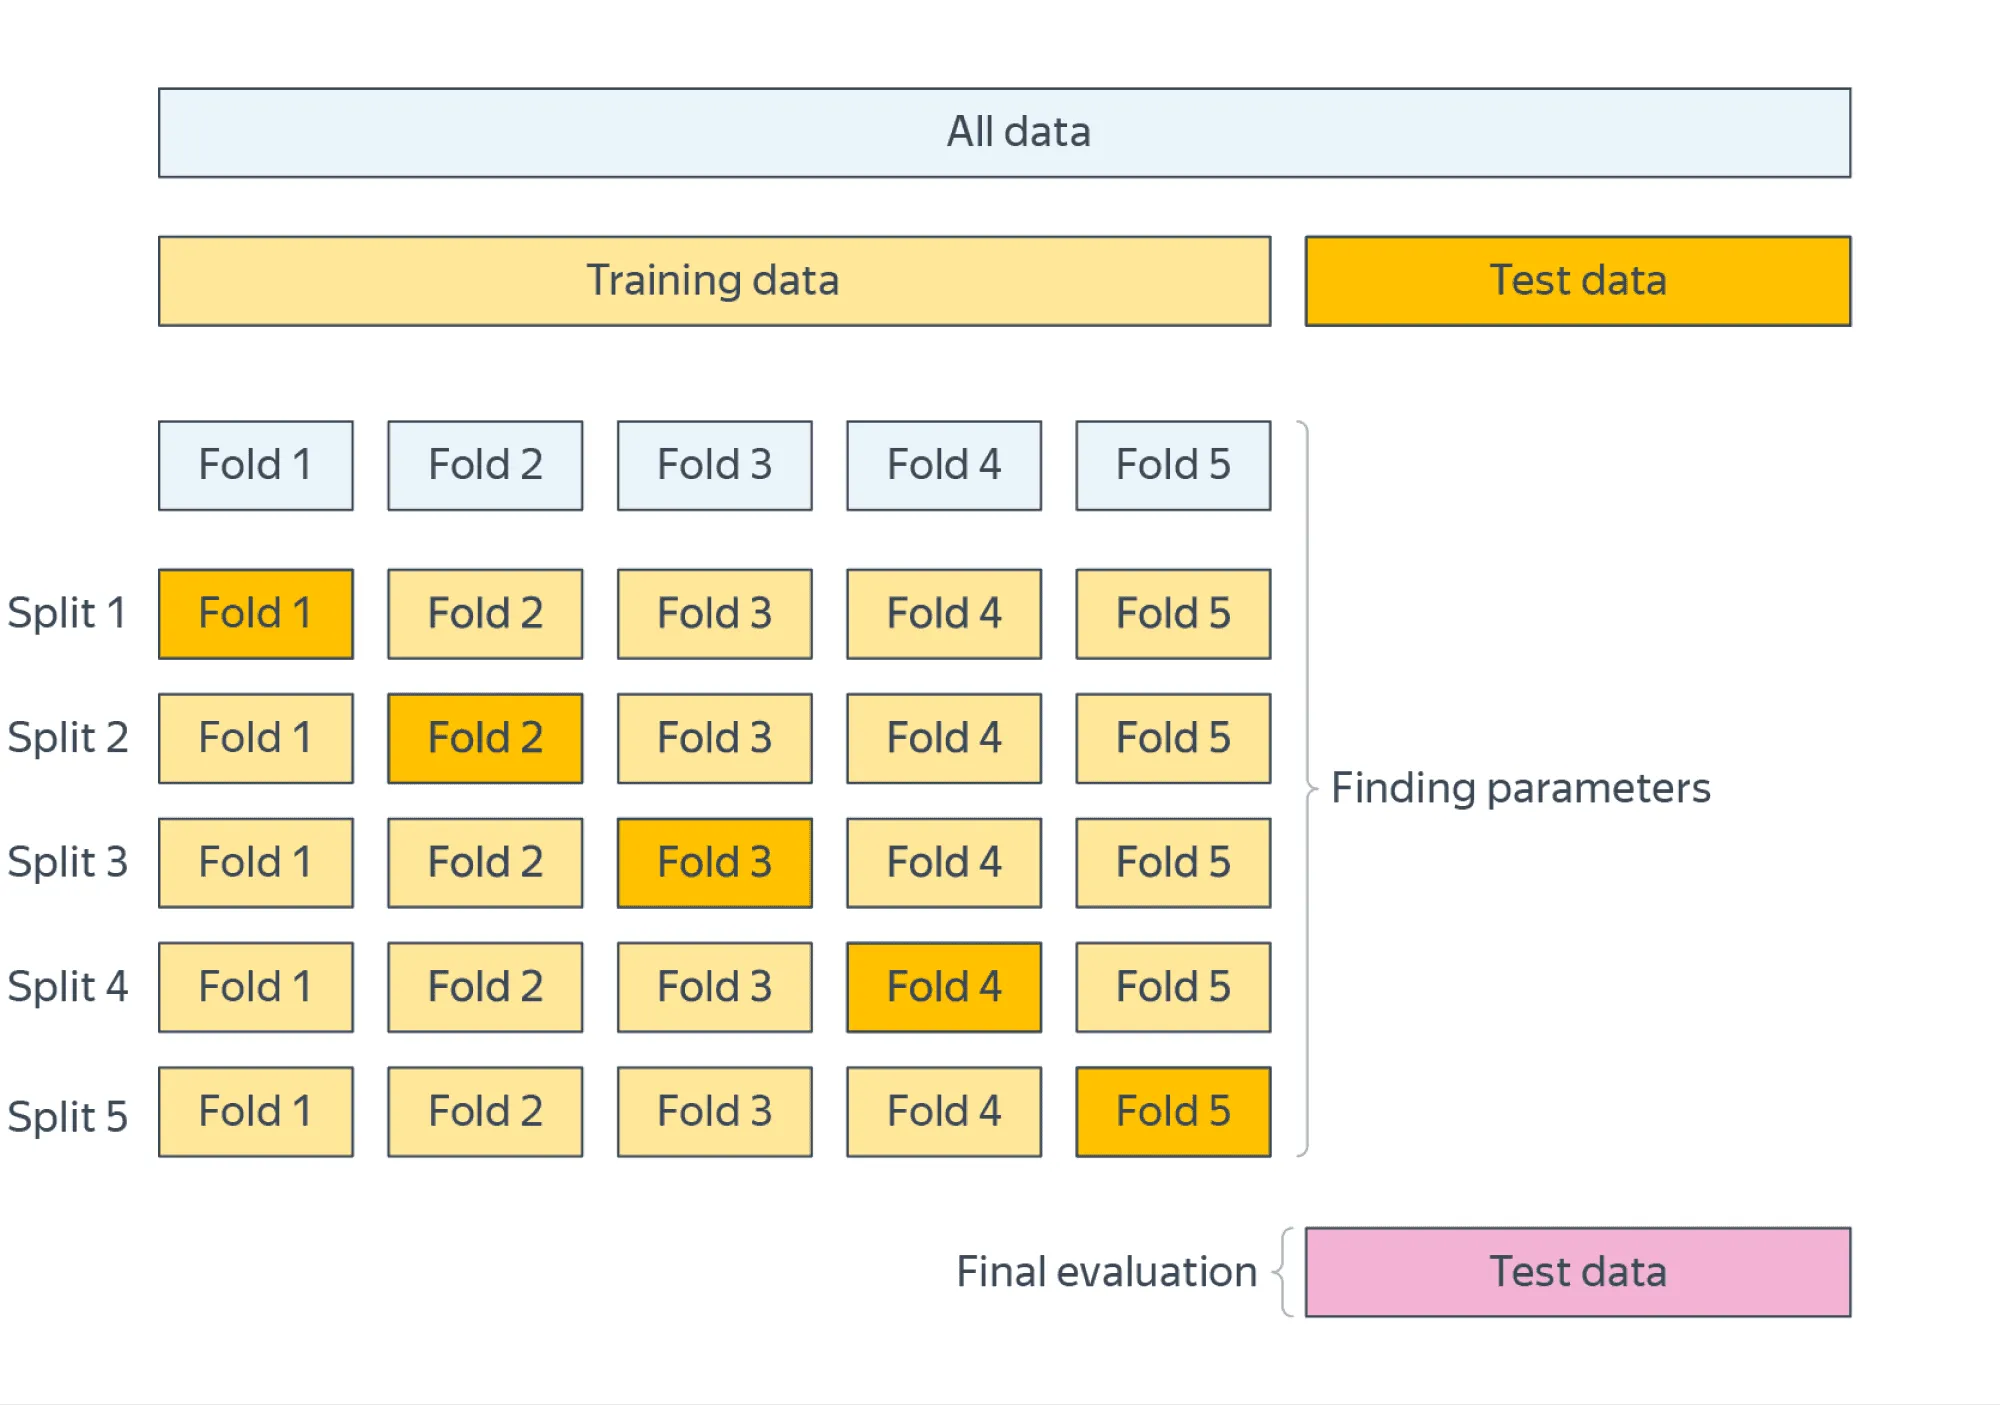
\includegraphics[width=1\textwidth]{img/cv_split.png}
	\end{frame}
	
	\begin{frame}
		\frametitle{Заключение}
		\begin{itemize}
			\item Метрики служат для сравнения обученных моделей
			\item Метрики должны отражать бизнес требования
			\item Функция потерь -- математическое приближение бизнес метрики
			\item Обучение модели, подбор гиперпараметров и оценка качества - на разных наборах данных
			
		\end{itemize}
	\end{frame}
	
	
\end{document}